\documentclass{article}
\title{Trabajo final IFC}
\author{Ignacio Loaiza   41205127-2}
\date{04/Sep/2014}
\usepackage{graphicx}
\usepackage[left=3cm, right=3cm, top=2.5cm, bottom=2.5cm]{geometry}
\usepackage[spanish]{babel}
\begin{document}
\begin{titlepage}

\newcommand{\HRule}{\rule{\linewidth}{0.5mm}}
\center 
 
\textsc{\LARGE UNIVERSIDAD NACIONAL AUT\'ONOMA DE M\'EXICO}\\[1.5cm] 
\textsc{\Large Facultad de Ciencias}\\[0.5cm] 
\textsc{\large Laboratorio de electr\'onica}\\[0.5cm] 
\HRule \\[0.4cm]
{ \huge \bfseries Pr\'actica II: Medici\'on de voltajes e instrumentaci\'on}\\[0.4cm]
\HRule \\[1.5cm]
\begin{minipage}{0.4\textwidth}
\begin{flushleft} \large
\emph{Alumno:}\\
Ignacio \textsc{Loaiza}
\end{flushleft}
\end{minipage}
~
\begin{minipage}{0.4\textwidth}
\begin{flushright} \large
\emph{Profesor} \\
Dr. Jos\'e\ Manuel \textsc{Alvarado Reyes}
\end{flushright}
\end{minipage}\\[3cm]
{\large 4 de Septiembre de 2014}\\[0.5cm]
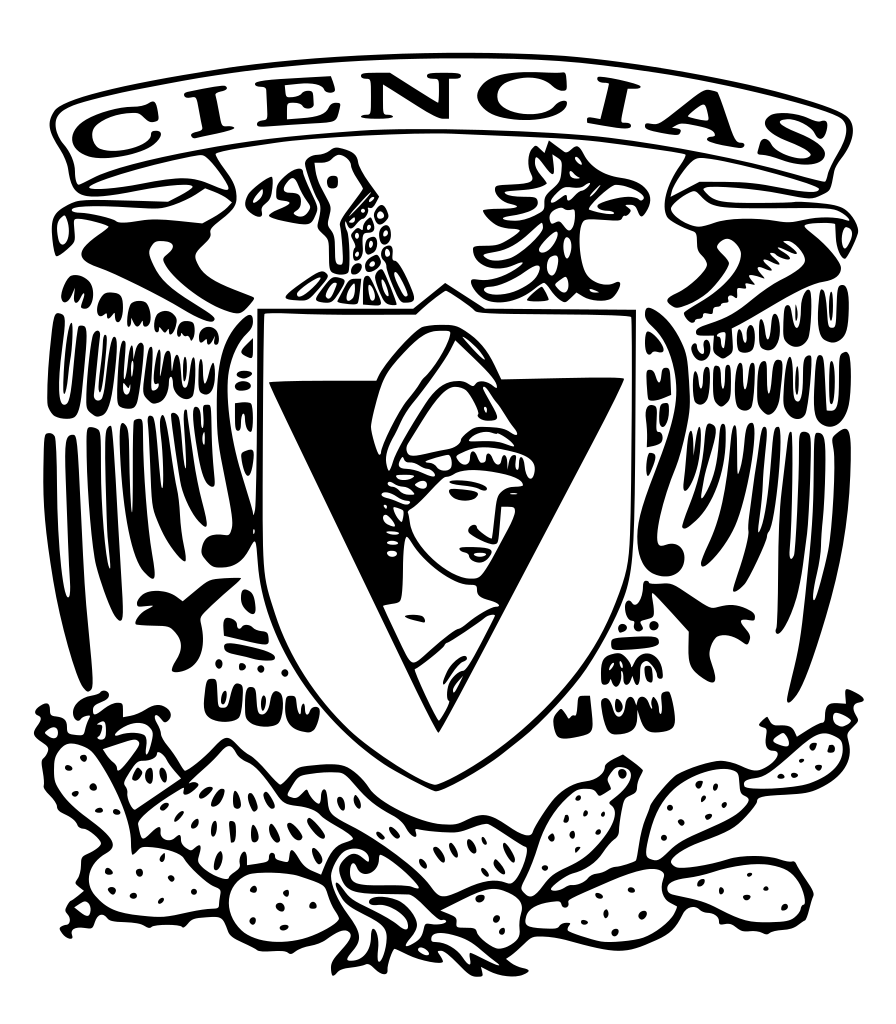
\includegraphics[width=6cm]{/home/nacho/Escuela/ciencias.png}\\[1cm]
\vfill
\end{titlepage}


\section{Resumen}
En esta pr\'actica se busc\'o\ familiarizarse con el concepto de voltaje, adem\'as de aprender a utilizar los aparatos del laboratorio, entendiendo sus limitantes. Para hacer esto se hicieron circuitos con fuentes distintas (simples, dobles y/o generadores de funciones) con arreglos de resistencias conectados a estas, y se midieron los voltajes en los circuitos utilizando mult\'imetros y el osciloscopio.

\section{Introducci\'on}
A lo largo de varios laboratorios se han usado los aparatos de electr\'onica para medir voltajes sin estar realmente bien familiarizados con el uso de los aparatos, as\'i\ como con el concepto de voltaje. Resulta natural hacer una pr\'actica para entender realmente qu\'e\ es el voltaje, as\'i\ como aprender a utilizar de forma correcta los instrumentos, permiti\'endonos experimentar de la forma correcta con un buen entendimiento de la electr\'onica.

\section{Marco Te\'orico}
Sea un circuito con una resistencia $R$ el cual es sometido a un voltaje de $V$ con una corriente $I$, se tiene entonces que, seg\'un la Ley de Ohm:
\begin{equation}
V=RI
\end{equation}
La ley de las mallas de Kirchhoff nos dice que, en una malla, se tiene que:
\begin{equation}
\sum V_i=0
\end{equation}
D\'onde $V_i$ son los voltajes que se tienen en una malla. \\ 
Para aplicar esta ley no hay que olvidar los sentidos distintos que tiene un voltaje (por lo general se toman en un sentido los voltajes de los elementos que dan corriente y en otro sentido de los que la reciben). La ley tambi\'en se puede reescribir entonces como:
\begin{equation}
\sum V_G=\sum V_R
\end{equation}
D\'onde $V_G$ son los elementos que generan la corriente y $V_R$ los que la reciben.
Se puede ver un esquema de la ley en la siguiente figura:
\begin{center}
\includegraphics[width=4cm]{malla.png}
\end{center}
\begin{center}
Figura 1: Esquema de la ley de las mallas.
\end{center}

La ley de los nodos de Kirchhoff dice que, en un nodo:
\begin{equation}
\sum I_i=0
\end{equation}
D\'onde $I_i$ son las intensidades de la corriente que se tienen en un nodo. Esta ley tambi\'en se puede escribir como:
\begin{equation}
\sum I_E=\sum I_S
\end{equation}
D\'onde $I_E$ son las corrientes entrantes al nodo y $I_S$ son las salientes.
Se puede ver un esquema de esta ley en la siguiente figura:
\vspace{5cm}
\begin{center}
Figura 2: Esquema de la ley de los nodos.
\end{center}
Al conectar un mult\'imetro o alg\'un otro tipo de medidor en el circuito, de estas dos leyes se deduce entonces que:
\begin{itemize}
\item Si se quiere medir el voltaje, hay que conectar el medidor en paralelo, haciendo una malla en la cual los \'unicos elementos son el medidor y el elemento cuyo voltaje se quiere medir. De la ley de las mallas se deduce entonces que el voltaje que indica el medidor es el voltaje del elemento
\item Si se quiere medir la corriente, hay que conectar el medidor sobre la misma rama del elemento que se quiere medir, de forma que no haya ning\'un nodo entre el medidor y el elemento. De la ley de los nodos se sigue entonces que la corriente que pasa a trav\'es del medidor es la misma que pasa a trav\'es del elemento.
\end{itemize}
La potencia que pasa por un elemento se puede obtener a partir de la f\'ormula siguiente:
\begin{equation}
P=VI
\end{equation}
D\'onde $V$ es el voltaje al que est\'a\ sometido e $I$ es la corriente que pasa por el elemento. La potencia, como su nombre lo indica, est\'a\ relacionada con que tanta energ\'ia est\'a\ pasando por el elemento, y si se pasa demasiada potencia por un elemento que no la soporte este se puede quemar. \\ \\ 
Al medir un voltaje, hay que fijarse qu\'e\ tipo de voltaje se est\'a\ midiendo, ya que existen varios tipos:
\begin{enumerate}
\item El voltaje DC o de corriente continua $V_{DC}$. El n\'umero que se le asigna a este voltaje es el valor constante que toma a lo largo del tiempo.
\item El voltaje pico (en corrientes alternas) $V_p$. El n\'umero que se le asocia a este voltaje corresponde al valor m\'aximo que alcanza el voltaje alterno con respecto al tiempo.
\item El voltaje pico pico (en corrientes alternas) $V_{pp}$. Este voltaje est\'a\ dado por la diferencia de voltaje entre un m\'aximo y un m\'inimo del voltaje, y cumple entonces que $V_{pp}=2V_p$.
\item El voltaje RMS (en corrientes alternas) $V_{rms}$. Este voltaje refleja cuanto voltaje van a "\textit{sentir}" los elementos, siendo un promedio del voltaje de corriente alterna. Se tiene que este voltaje cumple con la relaci\'on $V_{rms}=\frac{1}{\sqrt{2}}V_p$.
\end{enumerate}
Se puede ver un esquema de los distintos tipos de voltaje a continuaci\'on:
\vspace{5cm}
\begin{center}
Figura 3: Esquema de los distintos tipos de voltaje.
\end{center}
En un voltaje alterno, se tiene entonces que la frecuencia $\nu$ \'o\ $f$ est\'a\ dada por la siguiente f\'ormula:
\begin{equation}
\nu=f=\frac{1}{T}
\end{equation}
D\'onde $T$ es el periodo de oscilaci\'on, sea el tiempo que le toma al voltaje completar un ciclo. \\ \\
La transformada de Fourier de una funci\'on peri\'odica nos manda a un espacio de frecuencias, en el cual en vez de graficar a voltaje con respecto al tiempo, se tiene que se grafican las amplitudes de las frecuencias con respecto a las frecuencias. Esta es entonces una herramienta muy \'util en el estudio de voltajes alternos, ya que permite estudiar de qu\'e\ frecuencias est\'a\ compuesto, as\'i\ como las amplitudes de estas frecuencias. El \textbf{ancho de banda} $WB$ \'o\ $\Delta WB$ est\'a\ relacionado con el rango de frecuencias en el cual hay voltaje, y se obtiene de la siguiente ecuaci\'on:
\begin{equation}
\Delta BW=BW=f_2-f_1
\end{equation}
D\'onde $f_1$ es la frecuencia m\'inima con una amplitud menor a la amplitud m\'axima por $3dB$, y $f_2$ es la frecuencia m\'axima con una amplitud menor a la m\'axima por $3dB$. Este concepto sirve entonces para saber en qu\'e\ rango de frecuencias est\'a\ el voltaje, eliminando cualquier ruido no deseado de su valor. \\ \\
La impedancia $Z=[Omhs]=[\Omega]$ de un aparato electr\'onico es su resistencia interna. Por lo general, los instrumentos que dan se\~nal tienen impedancias peque\~nas, mientras que los que reciben se\~nal tienen impedancias grandes. 


\section{Experimentaci\'on}
Este experimento se parte en tres grandes secciones:
\begin{enumerate}
\item Instrumentaci\'on
\item Impedancias
\item Frecuencias
\end{enumerate}
Cabe notar que todas las secciones est\'an relacionadas con la medici\'on de voltaje y el uso correcto de la instrumentaci\'on.

\subsection{Instrumentaci\'on}
\subsubsection{Materiales}
Los materiales utilizados en esta pr\'actica fueron:
\begin{itemize}
\item Mult\'imetros
\item Fuente DC simple
\item Fuente DC doble
\item Generador de funciones
\item Transformador
\item Osciloscopio
\end{itemize}

\subsubsection{M\'etodo experimental}
Se conectaron a los distintos tipos de fuentes (fuente simple, fuente doble, generador de funciones y transformador) primero al mult\'imetro en modo voltaje y luego al osciloscopio, y se estudiaron los voltajes de salida en los medidores al variar los voltajes de salida en las fuentes, de forma que se busc\'o\ entender qu\'e\ bot\'on regula qu\'e\ cosa. \\
Cabe notar que, para las mediciones con el osciloscopio, antes de hacer la medici\'on hay que establecer la tierra del osciloscopio en cero, ya que sino las mediciones no tendr\'an sentido. \\
Tambi\'en hay que subrayar que, al encender la fuente simple, hay que verificar antes que esta est\'e\ en el voltaje m\'inimo y la corriente m\'axima, moviendo nada m\'as el regulador de voltaje. La corriente al m\'aximo se establece para que, si un circuito requiere m\'as corriente debido a su resistencia y al voltaje suministrado, entonces este la va a tomar de la fuente, y si la corriente de la fuente no est\'a\ al m\'aximo entonces esta se puede quemar, ya que el circuito toma "\textit{a la fuerza}" la corriente. \\
Finalmente, para el generador de funciones tambi\'en se estudi\'o\ c\'omo utilizar la funci\'on \textbf{sweep} (barrido de frecuencias) utilizando el osciloscopio en la salida del generador, y tambi\'en en la salida del sweep (la cual nos muestra un voltaje asociado con el barrido llamado rampa del barrido). Adem\'as, tambi\'en se estudi\'o\ la funci\'on \textbf{offset} del generador de funciones.
\subsubsection{Resultados de Instrumentaci\'on}

\subsubsection*{Fuente simple:}
La fuente simple de DC tiene tres salidas: la positiva, la negativa y la de tierra. Se conectaron los cables de salida en el positivo y el negativo. Al hacer variar el voltaje de salida, en el osciloscopio se pudo ver c\'omo variaba el voltaje de acuerdo a lo que mostr\'o\ el \textit{display} de la fuente. Se midi\'o\ el mismo voltaje continuo en el osciloscopio que en el mult\'imetro, teniendo un voltaje de corriente continua $V_{DC}$ a la salida.

\subsubsection*{Fuente doble:}
Esta fuente no es variable y tambi\'en tiene tres salidas: la positiva, la tierra y la negativa. Al conectar los medidores, se observ\'o\ un voltaje continuo. Entre la salida positiva y la de tierra hubo un voltaje de $+12V_{DC}$ al igual que entre la tierra y el negativo (teniendo un voltaje de $-12V_{DC}$ entre el negativo y la tierra). Finalmente, al medir el voltaje entre el positivo y el negativo se midi\'o\ un voltaje de $+24V_{DC}$.

\subsubsection*{Transformador:}
El transformador tambi\'en tiene tres salidas, sean la $1$, $2$ y $3$. Los voltajes que se midieron con el mult\'imetro fueron los siguientes:
$$V_{12}=12.48V_{rms}, \ \ \ V_{13}=25.83V_{rms}, \ \ \ V_{23}=12.99V_{rms};$$
Mientras que los valores medidos por el osciloscopio fueron:
$$V_{12}=18V_p, \ \ \ V_{13}=35.8V_p, \ \ \ V_{23}=18V_p.$$

\subsubsection*{Generador de funciones:}
Se conectaron los medidores a la salida del generador de funciones. Cabe notar que, al poner una salida de $5Hz$ del generador, el mult\'imetro no fu\'e\ capaz de medir el voltaje, obteniendo valores variantes y claramente err\'oneos. Se utiliz\'o\ entonces una frecuencia de $5kHz$, y se fu\'e\ variando la amplitud de la se\~nal de forma que se obtuvieron los siguientes valores:
\begin{center}
\begin{tabular}{||c|c||}
\hline
Voltaje pico [$V_p$] & Voltaje RMS [$V_{rms}$] \\ \hline
1 & 0.725 \\ \hline
2 & 1.378 \\ \hline
3 & 2.092 \\ \hline
4 & 2.816 \\ \hline
5 & 3.434 \\ \hline

\end{tabular}
\end{center}
\begin{center}
Tabla 1: Valores de los voltajes pico y RMS obtenidos para el generador de funciones a $5Khz$.
\end{center}
Tambi\'en hay que decir que, para los $5kHz$, las frecuencias en el osciloscopio se pudieron medir en la escala correcta, pero al colocar una escala mucho mayor de tiempo se obtuvo un efecto en el cual el osciloscopio midi\'o\ una frecuencia de $18Hz$. \\ \\
La funci\'on de \textbf{sweep} hace un barrido de frecuencias, lo cual quiere decir que va haciendo variar a la frecuencia. Con la opci\'on "sweep-rate" se controla que tan seguido se hacen los barridos (sea la frecuencia de la rampa de barrido), y con "stop freq" se controla hasta que frecuencia va a llegar el barrido (sea la amplitud de la rampa de barrido). A continuaci\'on se puede observar c\'omo afecta la rampa de barrido a la frecuencia del voltaje dado por el generador de funciones:
\begin{center}
\includegraphics[width=8cm]{sweep.jpg}
\end{center}
\begin{center}
Figura 4: Variaci\'on del voltaje de salida del generador de funciones con el sweep y rampa de barrido.
\end{center}
Al utilizar la funci\'on \textbf{offset}, el generador "sube o baja" el voltaje de salida (sea que en vez de variar entre $V_p$ y $-V_p$, ahora var\'ia entre $V_p+Off$ y $Off-V_p$, d\'onde $Off$ es el voltaje del offset). Cabe notar que, si se pon\'ia al osciloscopio en modo de medici\'on de corriente cont\'inua (DC), se pod\'ian observar estos desplazamientos, mientras que en el modo de corriente alterna (AC), el osciloscopio ignora cualquier tipo de desplazamiento, nada m\'as mostrando la componente que var\'ia con respecto al tiempo del voltaje.

\subsubsection{Discusi\'on de Instrumentaci\'on}
Se midieron los voltajes cont\'inuos para la fuente simple como se esperaba. Para la fuente doble, se puede concluir que, tomando la rama de la tierra como el voltaje cero, la salida positiva est\'a\ a $+12V_{DC}$ y la negativa a $-12V_{DC}$. \\
Para el transformador, se puede concluir que la salida de enmedio es su tierra. Tomando a esta salida como la referencia a $0V$, se tiene que las otras salidas est\'an a $12V_{rms}$, sea a aproximadamente $17V_p$. Adem\'as, estos voltajes est\'an en fase y tienen signos opuestos, de forma que cuando se toma el voltaje entre las salidas $1$ y $3$ se obtienen $24V_{rms}$, sea $34V_p$. \\
Para el generador de funciones, cabe destacar que se pudo observar uno de los l\'imites del mult\'imetro, ya que este no pudo medir de forma correcta el voltaje cuando la frecuencia era menor a $50Hz$, midiendo m\'as y m\'as precisamente seg\'un fu\'e\ aumentando la frecuencia. Se pudo adem\'as observar c\'omo, en la rampa del barrido, la amplitud controla el rango de frecuencias en el cual se va a hacer el barrido, mientras que la frecuencia controla la frecuencia con la que se hace el barrido.

\subsection{Impedancias}
\subsubsection{Materiales}
Los materiales utilizados fueron:
\begin{itemize}
\item Fuente simple DC
\item Cable de toma de corriente a caimanes
\item Resistencias variadas
\item Mult\'imetro
\item Osciloscopio
\end{itemize}

\subsubsection{M\'etodo experimental}
La primera parte del experimento consisit\'o\ en, utilizando la toma de la corriente (medida a $125.4V_{rms}$) \'o\ la fuente simple, hacer pasar corrientes por resistencias. Calculando la potencia que va a pasar por la resistencia a partir de las f\'ormulas $(1)$ y $(6)$, se obtiene que la potencia que va a haber en la resistencia es de:
$$P=VI=V\frac{V}{R}=\frac{V^2}{R}$$
Con $V=cte$ tenemos que la potencia var\'ia de la forma $1/R$. Se utilizaron entonces varias resistencias, haciendo pasar para algunas potencias m\'as grandes de las que aguantan. \\
La segunda parte de este experimento consisit\'o\ en observar los efectos de la impedancia. Para hacer esto, se conectaron resistencias que se fueron cambiando a la fuente simple, y se midi\'o\ el voltaje en esta cuando el voltaje de salida de la fuente marcaba $10V$ (DC).

\subsubsection{Resultados de Impedancias}
Para la primera parte del experimento, se utilizaron resistencias de $22\Omega$ para la toma de corriente, y resistencias de $10\Omega$, $3.4\Omega$ y de $1\Omega$ para la fuente simple con salida de $10V$ (DC), todas con una potencia menor o igual a $20W$. Las resistencias de $22$ y de $10$ Ohms se quemaron, mientras que las de $3.6$ y $1$ Ohms causaron una baja en el voltaje de la fuente, la cual marc\'o\ corto circuito (CC), y fueron desconectadas r\'apidamente antes de causar da\~nos permanentes en el equipo. \\ \\
Para la segunda parte, se utilizaron resistencias de $2.2M\Omega$ y de $22M\Omega$. Para la de $2.2M\Omega$, el voltaje medido por el osciloscopio fu\'e\ de $10.063V$ (DC), mientras que el voltaje medido por el mult\'imetro fu\'e\ de $4.523V$. Para la resistencia de $22M\Omega$, los voltajes medidos fueron de $2.386V$ para el osciloscopio y de $0.420V$ para el mult\'imetro.

\subsubsection{Discusi\'on de Impedancias}
En la primera parte, la resistencia de $22\Omega$ se quem\'o\ ya que la potencia a la que fu\'e\ sometida es de $P=(125.4)^2/22=710W$, siendo mucho mayor que la potencia m\'axima de $20W$ que aguanta. Para la resistencia de $10\Omega$, la corriente que requiri\'o\ fu\'e\ de $I=V/R=1A$ (la fuente simple tiene un l\'imite de $1.5A$), y la potencia que pas\'o\ fu\'e\ de $P=VI=10W$. Siendo una resistencia de baja potencia ($0.25W$), se quem\'o\. Para la tercera y la cuarta resistencia (de $3.4$ y de $1$ Ohms respectivamente), la intensidad que requirieron fu\'e\ mayor que los $1.5A$ que puede dar la fuente, lo que caus\'o\ que la fuente entrara en corto circuito, disminuyendo su voltaje (para la 3 baj\'o\ hasta $5.4V$, y para la 4 baj\'o\ hasta $2.6V$). Esto tiene mucho sentido si se estudia la composici\'on de la "caja negra", la cual se ve de la siguiente forma:
\vspace{5cm}

\begin{center}
Figura 5: Modelo de la "caja negra" para la fuente simple.
\end{center} 
En este modelo $R_i$ es la resistencia interna \'o\ \textbf{impedancia} de la fuente. Cuando se le coloc\'o\ una resistencia muy peque\~na y requiri\'o\ m\'as corriente, entonces el voltaje en $R_i$ se volvi\'o\ significativo en el circuito, dando la baja de voltaje que se observ\'o\ poco antes de que marcara corto circuito. \\ \\
En la segunda parte, a pesar de que el osciloscopio midi\'o\ el voltaje de forma correcta para la primera resistencia, al colocar resistencias muy altas (las cuales inducen corrientes muy peque\~nas si se toma un voltaje constante de $V=10V$), se tuvo que los aparatos de medici\'on ya no pudieron medir de forma correcta el voltaje en la resistencia. Esto se debe a que, debido a la impedancia (o resistencia interna) de los aparatos de medici\'on, estos necesitan una corriente m\'inima para poder medir voltajes de forma correcta. La impedancia del osciloscopio es entonces m\'as chica que la del mult\'imetro, ya que permite medir voltajes con corrientes m\'as peque\~nas.

\subsection{Frecuencias}
\subsubsection{Materiales}
Se utilizaron los siguientes materiales:
\begin{itemize}
\item Generadores de frecuencias
\item Fuente simple
\item Sumador de voltajes con alimentaci\'on (fuente doble de DC)
\item Transformador
\item Osciloscopio
\end{itemize}

\subsubsection{M\'etodo experimental}
Se conect\'o\ al sumador de voltajes con su alimentaci\'on y a la salida con el osciloscopio. Despu\'es, se conectaron a los 3 generadores de funciones (o dos generadores y el transformador, o dos generadores y la fuente simple) entre la tierra y respectivamente una de las entradas de voltaje del sumador, como se ve en el esquema a continuaci\'on:
\vspace{6cm}
\begin{center}
Figura 6: Esquema de circuito de conecciones para el circuito del sumador de corrientes.
\end{center}
Se estuvieron cambiando los tipos de voltajes de entrada, observando las resultantes de la suma en el osciloscopio.

\subsubsection{Resultados de Frecuencias}
\subsubsection*{1:}
Se puso uno de los generadores a una frecuencia de $250Hz$ con $1V_p$, y se estuvo variando el voltaje de salida de la fuente simple de corriente cont\'inua. Se obtuvo un resultado id\'entico a cuando se utiliz\'o\ la funci\'on offset del generador de funciones, obteniendo un desplazamiento de la funci\'on (el cual s\'olo fu\'e\ visible para el osciloscopio en modo DC, no en modo AC).

\subsubsection*{2:}
Se conect\'o\ al transformador (salida a $63.49Hz$), baj\'andole el voltaje con un divisor de voltaje para no da\~nar al sumador (con un voltaje de entrada de $1.6V_p$ entonces), y se conect\'o\ un generador de funciones con un voltaje m\'as peque\~no. Primero se puso el generador de funciones a $300Hz$, obteniendo un voltaje de $300Hz$ montado sobre uno de $63.49Hz$ como se puede observar en la siguiente imagen:
\begin{center}
\includegraphics[width=7cm]{uno.jpg}
\end{center}
\begin{center}
Figura 7.1: Voltaje de alta frecuencia montado sobre voltaje de baja frecuencia en el sumador de voltajes.
\end{center}
Cuando se aument\'o\ la frecuencia del generador a $1kHz$ se obtuvo la siguiente imagen:
\begin{center}
\includegraphics[width=7cm]{dos.jpg}
\end{center}
\begin{center}
Figura 8: Voltaje de m\'as alta frecuencia montado sobre voltaje de baja frecuencia en el sumador de voltajes.
\end{center}
Y cuando sew disminuy\'o\ la frecuencia a $63Hz$ y se igual\'o\ el voltaje pico con el del transformador, se obtuvieron beatings como se puede ver en la figura a continuaci\'on:
\begin{center}
\includegraphics[width=7cm]{beats.jpg}
\end{center}
\begin{center}
Figura 9: Voltajes de frecuencias similares en el sumador de voltajes.
\end{center}

\subsubsection*{3:}
Se comenz\'o\ con dos generadores de funciones haciendo beatings a $60Hz$, y despu\'es se le coloc\'o\ sweep a uno de ellos. Se pudo observar como los beatings van desapareciendo seg\'un va avanzando el sweep, y vuelven a aparecer cuando este comienza. En la ventana de transformada de Fourier del osciloscopio (FFT) se ve\'ian dos picos cercanos (las frecuencias que hacen beatings), y uno de ellos se iba alejando poco a poco, hasta que desaparec\'ia y volv\'ia a aparecer junto al otro pico.

\subsubsection*{4:}
Se colocaron los tres generadores de funciones a frecuencias cercanas ($1.098kHz$, $1.100kHz$ y $1.630kHz$) a la misma amplitud, obteniendo la siguiente imagen en la transformada de Fourier:
\begin{center}
\includegraphics[width=7cm]{fourier1.jpg}
\end{center}
\begin{center}
Figura 10: Transformada de Fourier de la suma de 3 generadores de funciones.
\end{center}
Despu\'es se colocaron a $1$, $2$ y $4$ kHz, obteniendo una imagen similar pero con los picos m\'as alejados y colocados cada uno sobre la frecuencia correspondiente.

\subsubsection*{5:}
Con un s\'olo generador, se hizo un barrido muy r\'apido y se visualiz\'o\ la transformada de Fourier. Cuando el barrido no era lo suficientemente r\'apido, se pod\'ia ver un pico que se iba moviendo en el rango de frecuencias del barrido. Sin embargo, cuando el barrido fu\'e\ lo suficientemente r\'apido, se observ\'o\ todo un rango de frecuencias en la transformada de Fourier, pudiendo medir entonces el ancho de banda del barrido. Cabe notar que, cuando se aument\'o\ la frecuencia l\'imite del barrido (sea que el generador diera en algunos momentos frecuencias muy altas), se comenzaron a generar arm\'onicos de las frecuencias altas en la transformada de Fourier.

\subsubsection{Discusi\'on de Frecuencias}
Se pudo observar como el sumador de voltajes suma los voltajes desde el primer resultado. En la segunda serie de resultados, cabe notar como, cuando se suman un voltaje a baja frecuencia con uno de alta, el de alta frecuencia se monta sobre el de baja, teniendo que el de alta frecuencia va viajando sobre el de baja frecuencia, lo cual concuerda con la teor\'ia de suma de funciones sinusoidales. \\
Para las siguientes partes, se pudo ver c\'omo la funci\'on transformada de Fourier requiere cierto tiempo de integraci\'on, ya que, para barridos muy r\'apidos, ya no pudo visualizar el pico que se iba moviendo, visualizando entonces todo un rango de frecuencias en el que est\'a\ el voltaje. \\
Los arm\'onicos que se iban creando cuando se aument\'o\ mucho la frecuencia l\'imite del barrido son debidos a errores de los instrumentos, se puede entonces ver otra de las limitantes de la instrumentaci\'on: la frecuencia.


\section{Conclusi\'on}
A lo largo de toda esta pr\'actica, adem\'as de aprender a utilizar la instrumentaci\'on de forma correcta, se pudieron ver las limitantes de \'esta: la resistencia $R$ (parte de impedancias), la corriente $I$ (parte de impedancias), la potencia $P$ (parte de impedancias) y la frecuencia $f$ (parte de frecuencias). Hay que recalcar entonces la importancia de escoger de forma adecuada la instrumentaci\'on para el f\'in que se le piensa dar: no sirve de nada un osciloscopio que mida hasta muy altas frecuencias si se va a estar trabajando en el intervalo del audio (de $20Hz$ a $20kHz$), de la misma forma que hay que escoger la fuente adecuada en funci\'on de la resistencia y de la corriente que vaya a necesitar el circuito que va a alimentar. Adem\'as, se diferenciaron todos los tipos distintos de voltajes y qu\'e\ tipo de instrumento est\'a\ asociado con qu\'e\ tipo de voltaje (fuentes de DC con $V_{DC}$, generadores de funciones con todos los tipos de voltajes alternos, mult\'imetro con $V_{DC}$ y con $V_{rms}$, y osciloscopio con $V_{DC}$, $V_p$ y $V_{pp}$).


\section{Bibliograf\'ia}
\begin{enumerate}
\item \textit{Bit\'acora de laboratorio de electr\'onica 2015-1}, Ignacio Loaiza
\end{enumerate}

\end{document}
